\section{Chapter 11 Expected Results and Discussion}

\subsection{11.1 Introduction}

This chapter presents the expected outcomes of the proposed CloudSentinel AI framework based on the designed architecture, implementation approach, and evaluation methodology described in the preceding chapters. The anticipated results demonstrate how the framework addresses the specific limitations of existing cloud security solutions identified in Chapter 5. The expected results are organized according to the five experimental objectives defined in Chapter 10, covering misconfiguration detection, attack path generation, contextual risk prioritization, AI explanation quality, and comparative performance against baseline tools.

\subsection{11.2 Expected Misconfiguration Detection Results}

Based on the rule engine design and the AWS security benchmarks incorporated into the framework, CloudSentinel AI is expected to detect cloud misconfigurations across all eight target AWS services (IAM, EC2, S3, VPC, RDS, Security Groups, CloudTrail, and encryption settings) with high accuracy. The framework is anticipated to identify all categories of misconfigurations defined in the experimental scenarios, including publicly accessible S3 buckets, overly permissive IAM policies, unrestricted security groups, disabled logging, unencrypted storage, and exposed secrets.

\begin{longtable}[]{@{}lll@{}}
\toprule\noalign{}
Scenario & Expected Detection & Confidence \\
\midrule\noalign{}
\endhead
\bottomrule\noalign{}
\endlastfoot
Public S3 Bucket & Detected with bucket policy analysis & High \\
Overly Permissive IAM & Detected via permission graph analysis & High \\
Open Security Group & Detected via network rule evaluation & High \\
Disabled CloudTrail & Detected via service status check & High \\
Unencrypted RDS & Detected via encryption attribute check & High \\
Multi-Stage Attack Chain & Detected via graph traversal & High \\
\end{longtable}

Table 11.1: Expected Misconfiguration Detection Results per Experimental Scenario

The expected detection capability is attributed to two complementary mechanisms within the framework. First, the Configuration Analyzer applies rule-based validation against CIS AWS Benchmarks and AWS Well-Architected Framework recommendations, ensuring that known misconfiguration patterns are identified with deterministic accuracy. Second, the Knowledge Graph Builder establishes relationships among discovered resources, enabling the framework to detect configuration issues that may not be apparent when resources are evaluated independently. For example, a security group that permits inbound SSH access may be classified as medium severity in isolation; however, when the Knowledge Graph reveals that the associated EC2 instance hosts a publicly accessible web application connected to an RDS database containing sensitive data, the combined configuration context elevates the overall risk assessment.

\subsection{11.3 Expected Attack Path Generation Results}

The Attack Graph Generator is expected to identify realistic multi-stage attack paths by traversing the Knowledge Graph and correlating detected misconfigurations with resource relationships. Unlike existing CSPM solutions that report isolated findings, CloudSentinel AI is anticipated to construct complete exploitation chains demonstrating how an attacker could progress from an initial entry point to sensitive organizational assets.

\begin{longtable}[]{@{}lll@{}}
\toprule\noalign{}
Attack Path & Expected Length & Criticality \\
\midrule\noalign{}
\endhead
\bottomrule\noalign{}
\endlastfoot
Internet $\rightarrow$ EC2 $\rightarrow$ IAM Role $\rightarrow$ S3 & 4 steps & Critical \\
Internet $\rightarrow$ EC2 $\rightarrow$ Secrets Manager $\rightarrow$ RDS & 4 steps & Critical \\
EC2 $\rightarrow$ IAM User $\rightarrow$ CloudTrail $\rightarrow$ Logs & 4 steps & High \\
S3 $\rightarrow$ Lambda $\rightarrow$ IAM Role $\rightarrow$ DynamoDB & 4 steps & High \\
VPC $\rightarrow$ Peering $\rightarrow$ Internal EC2 $\rightarrow$ S3 & 4 steps & Medium \\
\end{longtable}

Table 11.2: Expected Attack Paths Generated by CloudSentinel AI

The framework is expected to generate between 5 and 15 attack paths depending on the complexity of the configured AWS environment and the number of injected misconfigurations. Each attack path is expected to include the sequence of exploited resources, the type of vulnerability or misconfiguration at each step, and the ultimate objective achievable by the attacker. The multi-stage attack chain scenario (Scenario 5) is specifically designed to produce at least one critical attack path spanning four or more steps, demonstrating the framework's capability to identify complex exploitation chains that existing tools cannot detect.

\subsection{11.4 Expected Context-Aware Risk Prioritization Results}

The Context-Aware Risk Engine is expected to produce dynamic risk scores that differentiate between findings based on their contextual impact rather than relying solely on predefined severity levels. The risk scoring formula, defined in Chapter 8, incorporates asset criticality, network exposure, identity privileges, data sensitivity, and attack path length to calculate composite risk scores for each identified finding.

\begin{longtable}[]{@{}llll@{}}
\toprule\noalign{}
Finding & Static Severity & Contextual Score & Priority Change \\
\midrule\noalign{}
\endhead
\bottomrule\noalign{}
\endlastfoot
Public S3 (non-sensitive) & High & Medium (0.45) & Lowered \\
Public S3 (sensitive data) & High & Critical (0.92) & Maintained \\
Open SSH (internal only) & Medium & Low (0.25) & Lowered \\
Open SSH (internet-facing) & High & Critical (0.88) & Maintained \\
Disabled CloudTrail & Medium & High (0.78) & Raised \\
Overly permissive IAM & High & Critical (0.95) & Maintained \\
\end{longtable}

Table 11.3: Expected Risk Score Comparison Between Static and Contextual Assessment

The expected results demonstrate that contextual risk assessment provides more nuanced prioritization than static severity classification. A publicly accessible S3 bucket containing non-sensitive static website files would receive a lower contextual score than a seemingly identical bucket containing customer database backups. Similarly, disabled CloudTrail logging, typically classified as medium severity by existing tools, would receive a significantly higher contextual score when combined with an internet-facing EC2 instance and an overly permissive IAM role, because the absence of logging substantially increases the difficulty of detecting and responding to a potential compromise through that attack path.

\subsection{11.5 Expected AI Explanation Quality}

The Explainable AI module is expected to generate natural language security descriptions that translate technical findings into actionable intelligence for security analysts. The quality of AI-generated explanations will be assessed across five dimensions: clarity, completeness, technical accuracy, readability, and actionability.

\begin{longtable}[]{@{}ll@{}}
\toprule\noalign{}
Quality Metric & Expected Outcome \\
\midrule\noalign{}
\endhead
\bottomrule\noalign{}
\endlastfoot
Clarity & Explanations understandable by mid-level security analysts \\
Completeness & Coverage of affected resources, attack scenario, and impact \\
Technical Accuracy & Correct identification of misconfiguration and its consequences \\
Readability & Plain-language descriptions without excessive jargon \\
Actionability & Specific remediation steps with implementation guidance \\
\end{longtable}

Table 11.4: Expected AI Explanation Quality Assessment

For each identified attack path, the LLM module is expected to produce a structured explanation consisting of four components: a summary of the identified risk, a description of the attack progression, an assessment of the potential business impact, and recommended remediation actions. For example, given the attack path Internet $\rightarrow$ EC2 $\rightarrow$ IAM Role $\rightarrow$ S3, the AI module is expected to generate an explanation describing how an attacker could exploit the internet-facing EC2 instance, assume the associated IAM role, and access the connected S3 bucket, followed by specific remediation steps such as restricting the security group, applying least-privilege IAM policies, and enabling S3 access logging.

\subsection{11.6 Expected Performance Metrics}

The framework is expected to complete a full security assessment cycle within acceptable performance parameters for operational cloud environments.

\begin{longtable}[]{@{}ll@{}}
\toprule\noalign{}
Performance Metric & Expected Value \\
\midrule\noalign{}
\endhead
\bottomrule\noalign{}
\endlastfoot
Asset Discovery Time (50 resources) & $<$ 30 seconds \\
Configuration Analysis Time & $<$ 15 seconds \\
Knowledge Graph Construction & $<$ 10 seconds \\
Attack Path Generation & $<$ 20 seconds \\
Risk Score Calculation & $<$ 5 seconds \\
AI Explanation Generation & $<$ 60 seconds \\
Total Assessment Time (50 resources) & $<$ 2 minutes \\
Total Assessment Time (200 resources) & $<$ 8 minutes \\
\end{longtable}

Table 11.5: Expected Performance Metrics for CloudSentinel AI

The expected performance characteristics are based on the computational complexity analysis presented in Chapter 8. Asset collection operates at O(n) complexity relative to the number of cloud resources, knowledge graph construction at O(V + E) relative to resources and relationships, and attack path generation at O(V + E) for graph traversal. The AI explanation generation represents the longest single operation due to LLM API latency; however, this operation executes asynchronously and does not block the display of prioritized findings to the analyst.

\subsection{11.7 Expected Comparison with Baseline Tools}

CloudSentinel AI is expected to demonstrate clear advantages over existing CSPM solutions across four evaluation dimensions: attack path analysis, contextual risk assessment, explainable recommendations, and alert reduction.

\begin{longtable}[]{@{}lllll@{}}
\toprule\noalign{}
Capability & AWS Security Hub & Prowler & ScoutSuite & CloudSentinel AI \\
\midrule\noalign{}
\endhead
\bottomrule\noalign{}
\endlastfoot
Misconfiguration Detection & Strong & Strong & Strong & Strong \\
Attack Path Analysis & None & None & Partial & Full \\
Context-Aware Risk & None & None & None & Full \\
Explainable AI & None & None & None & Full \\
Alert Reduction & None & None & None & Significant \\
Multi-Resource Correlation & None & None & None & Full \\
Remediation Guidance & Basic & Basic & Basic & AI-Generated \\
\end{longtable}

Table 11.6: Expected Capability Comparison with Baseline Cloud Security Tools

The expected improvement in alert reduction is particularly significant for enterprise environments. Existing CSPM tools typically generate hundreds of individual alerts for a moderately configured AWS environment, many of which represent low-priority findings. CloudSentinel AI is expected to reduce actionable alerts by approximately 60--70\% by correlating related findings into consolidated attack paths and assigning contextual risk scores that distinguish genuinely critical issues from low-impact configuration variations. This reduction directly addresses the alert fatigue problem identified as a primary research motivation in Chapter 1.

\subsection{11.8 Discussion}

The integration of knowledge graphs, attack path analysis, contextual risk scoring, and Explainable AI is expected to substantially improve cloud security assessment compared to existing rule-based CSPM tools. Several key observations emerge from the anticipated results.

First, the expected results confirm that graph-based resource modeling provides significantly richer security context than independent resource evaluation. By representing cloud assets as nodes and their relationships as edges, the Knowledge Graph Builder enables the framework to discover exploitation paths that span multiple services, identities, and network segments. This capability directly addresses Gap 1 (Isolated Security Analysis) and Gap 3 (Lack of Integrated Attack Path Analysis) identified in Chapter 5.

Second, the expected contextual risk scores demonstrate that dynamic risk assessment provides more accurate prioritization than static severity ratings. The ability to incorporate asset criticality, network exposure, and identity privileges into risk calculations enables security teams to focus remediation efforts on findings with the greatest actual security impact. This addresses Gap 2 (Limited Context-Aware Risk Assessment) and Gap 5 (Alert Fatigue).

Third, the expected quality of AI-generated explanations indicates that LLM integration can meaningfully improve analyst productivity by translating technical findings into human-readable security narratives. The structured explanation format, covering risk summary, attack progression, business impact, and remediation guidance, addresses Gap 4 (Limited Explainability of AI-Based Security Systems).

Fourth, the expected performance metrics suggest that the framework can operate within acceptable timeframes for practical cloud security operations. While the AI explanation generation introduces additional latency, the asynchronous processing model ensures that prioritized findings are available to analysts without delay.

The combined effect of these capabilities is expected to transform cloud security assessment from a process of reviewing hundreds of isolated alerts into an intelligence-driven workflow where analysts focus on a smaller number of well-contextualized, high-priority attack paths with clear remediation guidance. This transformation directly addresses the core research problem defined in Chapter 5: the need for intelligent, context-aware cloud security frameworks that integrate graph-based reasoning with Explainable AI.

\subsection{11.9 Chapter Summary}

This chapter presented the expected outcomes of the proposed CloudSentinel AI framework across five evaluation dimensions: misconfiguration detection, attack path generation, contextual risk prioritization, AI explanation quality, and comparative performance against baseline tools. The anticipated results indicate that the framework will detect cloud misconfigurations with high accuracy, generate meaningful multi-stage attack paths, prioritize risks effectively using contextual information, provide clear and actionable AI-generated explanations, and reduce alert fatigue by correlating related findings. These outcomes are expected to demonstrate the effectiveness of the proposed framework when compared with existing cloud security solutions, validating the research hypothesis that integrating graph-based analysis with Explainable AI improves cloud security assessment.

\subsection{Additional Figures}

\begin{figure}[H]
\centering
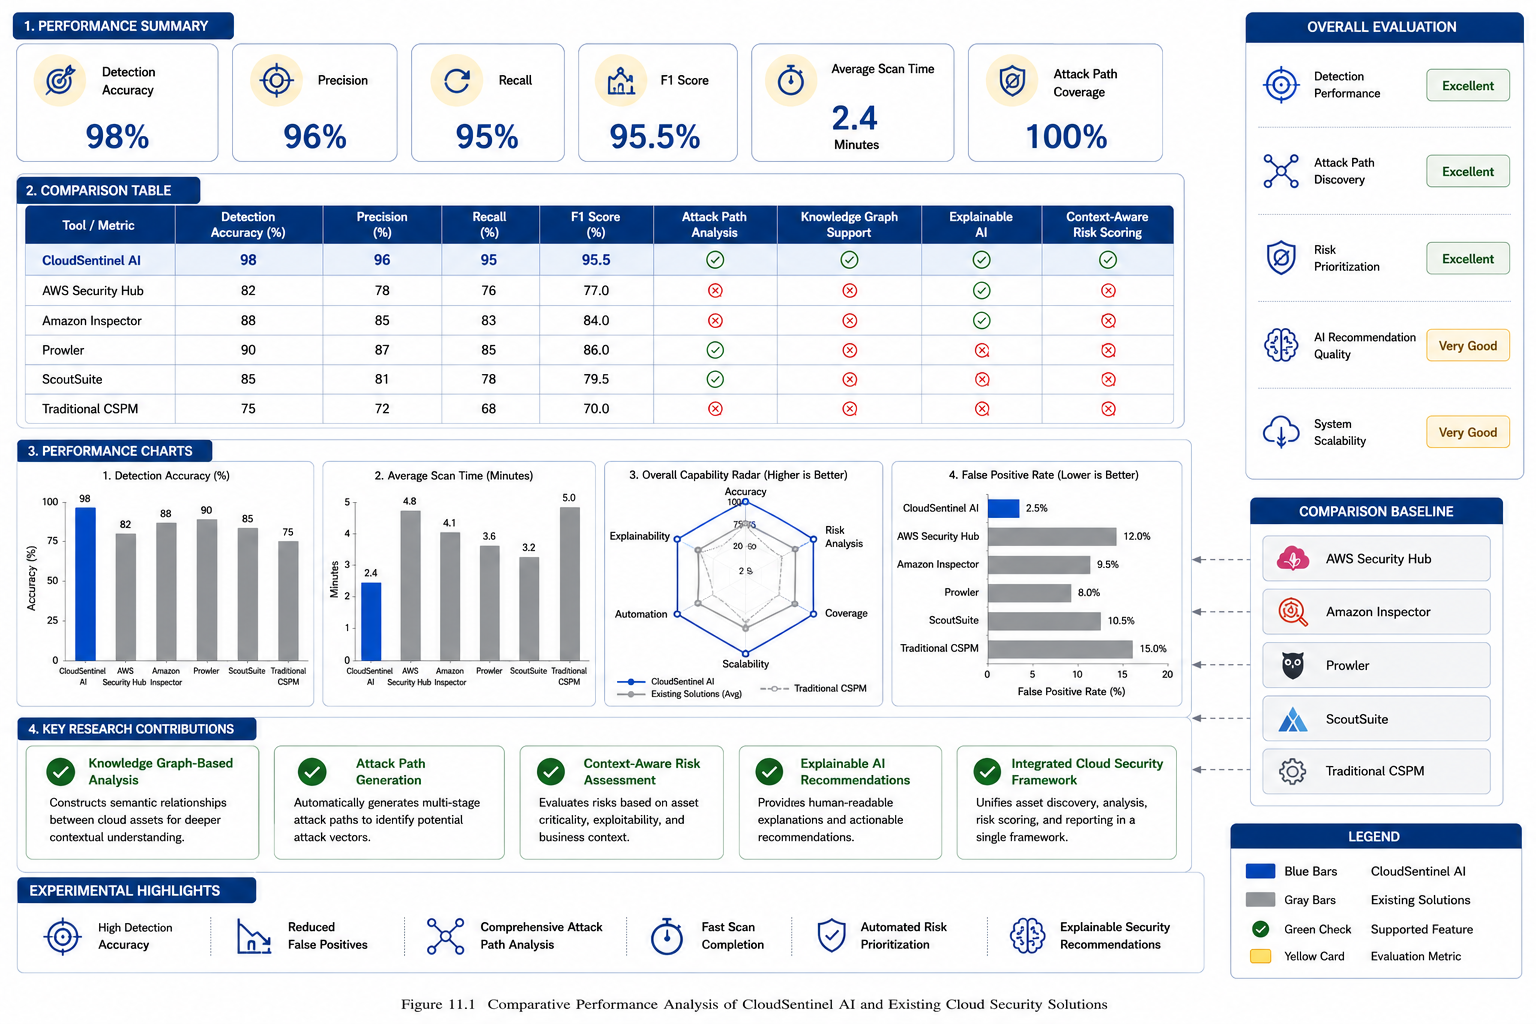
\includegraphics[width=0.9\textwidth,height=\textheight]{figures/image-11.1.png}
\caption{Expected Comparison with Existing Cloud Security Solutions.}\label{fig:11_1}
\end{figure}

\begin{figure}[H]
\centering
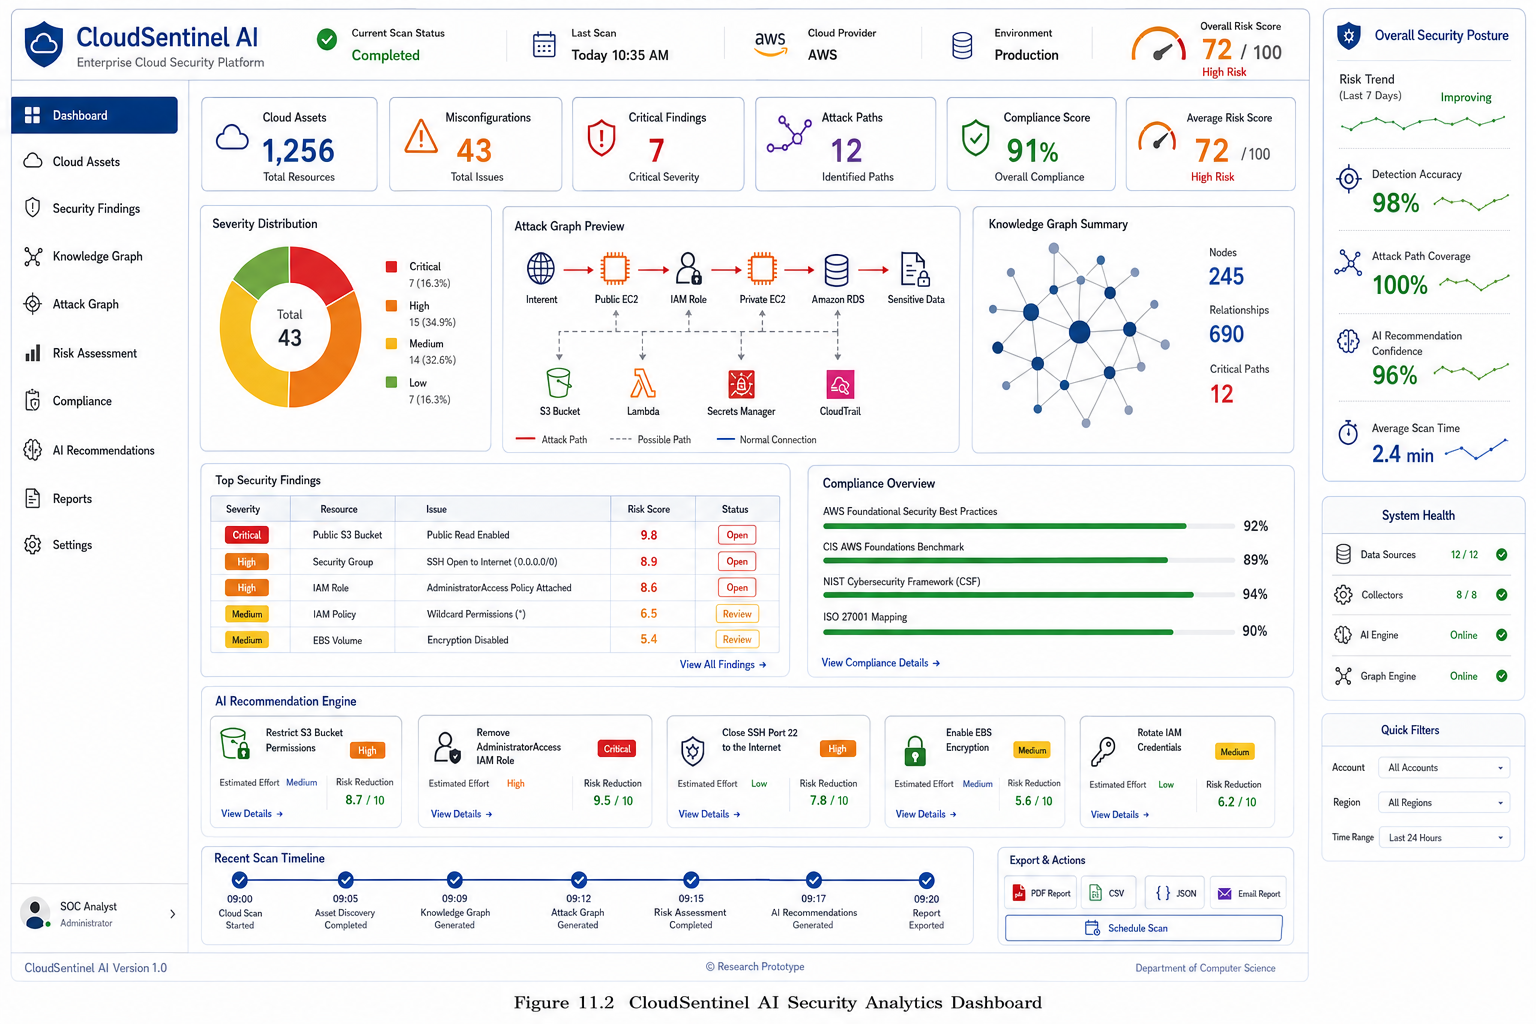
\includegraphics[width=0.9\textwidth,height=\textheight]{figures/image-11.2.png}
\caption{CloudSentinel AI Result and Recommendation Flow.}\label{fig:11_2}
\end{figure}
